\section{Line Integrals}
\subsection{Vector Fields}
This semester we started with vector functions, or functions from $\bbr\to\bbr^n$. Next, we studied surfaces, or functions from $\bbr^n\to\bbr$. We conclude the semester by studying vector fields, which are functions from $\bbr^n\to\bbr^n$. In particular, we'll be looking at vector fields from $\bbr^2\to\bbr^2$ and vector fields from $\bbr^3\to\bbr^3$.

\begin{definition}{Vector Field in $2$-Dimensions}
Let $\vcF$ be a function from $\bbr^2\to\bbr^2$ such that $$\vcF(x,y)=\bmat{P(x,y)\\Q(x,y)}=P(x,y)\vci+Q(x,y)\vcj.$$
We call $\vcF$ a vector field from $\bbr^2$ to $\bbr^2$.
\end{definition}

\begin{definition}{Vector Field in $3$-Dimensions}
Let $\vcF$ be a function from $\bbr^3\to\bbr^3$ such that $$\vcF(x,y,z)=\bmat{P(x,y,z)\\Q(x,y,z)\\R(x,y,z)}=P(x,y,z)\vci+Q(x,y,z)\vcj+R(x,y,z)\vck.$$
We call $\vcF$ a vector field from $\bbr^3$ to $\bbr^3$.
\end{definition}

As a note, we have actually already seen functions that were secretly vector fields. If you have some $f(x,y)=z$, then $$\nabla f=\bmat{f_x(x,y)\\f_y(x,y)} $$ is a 2-dimensional vector field.

Vector fields are often graphed by taking the domain, then picking some arbitrary points in the domain and drawing the resulting vector of that coordinates at that point in the domain. That is, to graph the vector field $$\vcF(x,y)=\bmat{-y\\x} $$ we would plot the vector $\bmat{-1\\1}$ at $(1,1)$, the vector $\bmat{-2\\1}$ at $(1,2)$ and so on and so forth. We often scale the vectors that we plot for clarity.

\begin{example}{A 2-Dimensional Vector Field}
Let $$\vcF(x,y)=\bmat{-y\\x}.$$ A plot of this vector field \href{https://doc.sagemath.org/html/en/reference/plotting/sage/plot/plot_field.html#}{generated using SageMath} at \href{https://sagecell.sagemath.org/}{SageMathCell} with the code
\vspace{1em}
\begin{verbatim}
x,y = var('x y')
plot_vector_field((-y,x), (x,-3,3), (y,-3,3))
\end{verbatim}
\vspace{1em}
\hypertarget{curl2}{is below:}
\vspace{1em}
\begin{center}
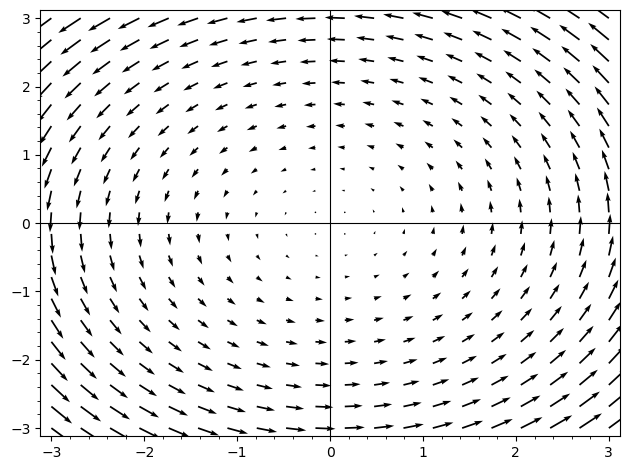
\includegraphics[scale=0.5]{Figures/vfieldex1}
$$\vcF(x,y)=\bmat{-y\\x} $$
\end{center}
\end{example}

\begin{example}{A Gradient Vector Field}
Let $f(x,y)=\sqrt{1-x^2-y^2}$. You should recognize this surface as the top half of the sphere with radius 1. But we can find $\nabla f$ and plot that as a $2$-dimensional vector field.
\begin{align*}
\nabla f=&\bmat{\delx{}(\sqrt{1-x^2-y^2})\\ \dely{}(\sqrt{1-x^2-y^2})}\\
=&\bmat{-\frac{x}{\sqrt{1-x^2-y^2}}\\-\frac{y}{\sqrt{1-x^2-y^2}}}.
\end{align*}
Then we can graph $\nabla f$ as a vector field:
\vspace{1em}
\begin{center}
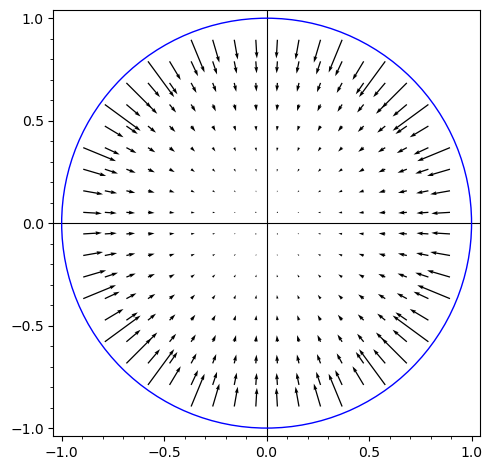
\includegraphics[scale=0.5]{Figures/gradvfieldex}\\
Gradient Vector Field for $f(x,y)=\sqrt{1-x^2-y^2}$.
\end{center}
\vspace{1em}
When referring to a vector field that comes from the gradient of a function, that is some $\vcF=\nabla f$, then $\vcF$ is the \textbf{gradient field} and $f$ is the \textbf{potential function}. If $\vcF$ is a vector field such that there exists some $f$ such that $\vcF=\nabla f$, then we say that $\vcF$ is a \textbf{conservative} vector field.
\end{example}

\begin{exercise}{Vector Fields}
For the following vector fields, generate a graph that has at least 5 vectors. You choose the points!
\vspace{1em}
\begin{enumerate}
\item $\vcF(x,y)=\bmat{2x\\-2}$.
\vspace{1em}
\item $\vcF(x,y)=\bmat{y-1\\x+y}$.
\end{enumerate}
\end{exercise}

\begin{exercise}{Gradient Vector Fields}
For the following functions, give the associated gradient vector field.
\vspace{1em}
\begin{enumerate}
\item $f(x,y)=y^2\cos(2x-y)$.
\vspace{1em}
\item $f(x,y,z)=xze^{y}$.
\end{enumerate}
\end{exercise}
